% Deployment chapter continued
\section{Infrastructure from 5,000 feet}
Now, following up from section \ref{infra10k}, the 2nd private subnet is the place where the crawler
resides.
\begin{figure}[h!]
  \centering
  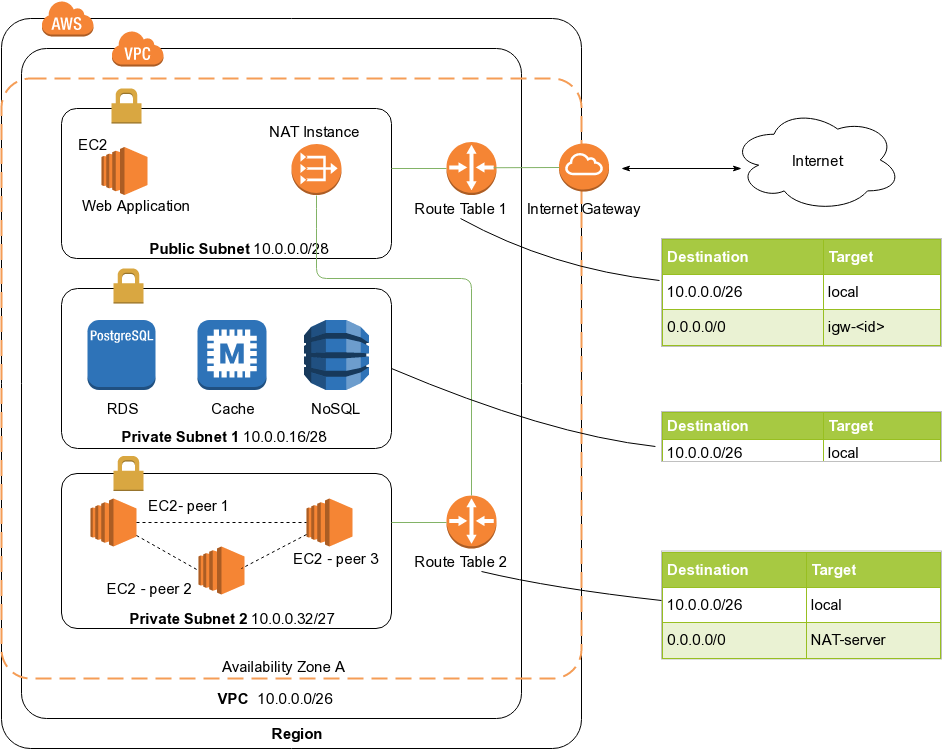
\includegraphics[width=20cm,height=12cm,keepaspectratio]{../media/crawler/aws-deploy-5k-feet.png}
  \caption{Whirlpool infrastructure with Route tables, NAT}
  \label{fig:infra5k}
\end{figure}

\noindent
According to figure \ref{fig:infra5k}, Each subnet is assigned a default route tables. In order for crawler
subnet to allow outbound traffic, a NAT instance is deployed on public subnet. NAT forwards traffic form instances to the internet and and send the response for corresponding request back to the instances.
It wont allow outside clients to initiate connections with instances in crawler subnet. Now the public subnet consists of one application server(EC2) and a NAT instance. The custom route(shown in route table 2)  is created and attached to crawler subnet. The custom rule directs the traffic originated within any of the private subnet peers matching subnet mask \ipAddress{0.0.0.0/0} to NAT server.
\\
\\
At this stage, the public subnet is not really public unless a Internet Gateway(IGW) is attached. After creating a Internet Gateway(IGW), a custom route(show in route table 1) is created and attached to the public subnet. This will scope all packets matching \ipAddress{0.0.0.0/0} route to IGW. The traffic from private
crawler subnet will flow to NAT Instance and then to the IGW. The NAT will translate back-and-forth source
and destination IPs of private instances.
\\
\\
The data store private subnet will contain RDS instance(PostgreSQL as part of the implementation). The
extracted data is hosted in DynamoDB which is a NoSQL variant. One good thing about DynamoDB is its
MongoDB compatible - the query language interface is blurred according to the recent announcement by AWS at
the time of this writing.

% note - here expand on EC2, RDS, cache, NoSQL, NAT computing specifications
\section{AWS resources Cost Estimation}
The below table provides approximate monthly billing information of AWS resources used by this project to build, test, and run experiments. The calculation was performed using AWS monthly calculator. At the time of
this writing, the author is enrolled is 12-month AWS Free tier access which discounts most of the services
the crawler system leverages.


\begin{figure}[h!]
  \centering
  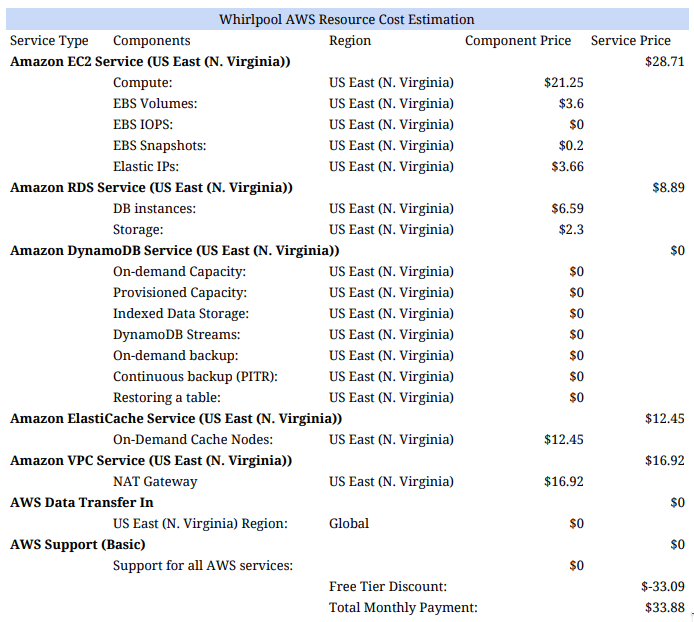
\includegraphics[width=20cm,height=12cm,keepaspectratio]{../media/crawler/aws-cost-estimate.png}
  \caption{AWS Monthly Expenses}
  \label{fig:awscost}
\end{figure}

Under Amazon EC2 services, each crawler node sits on a EC2 instance which is t2.micro - 1GiB RAM coupled
with Elastic Block Storage(EBS) volume of 5 GiB has approx. 5o\% utilization. Therefore a A 3-node crawler, will have 3x t2.micro and 3x 5 GiB EBS volumes.
\\
\\

\pagebreak